\documentclass{beamer}
\usepackage{amsmath}
\usepackage{amssymb}
\usepackage{bm}
\usepackage{extramarks}
\usepackage{amsfonts}
\usepackage{amsthm}
\usepackage{array}
\usepackage{xy}
\usepackage{multicol}
\usepackage{hyperref}
\usepackage{float}
\usepackage{subfig}
\usepackage{graphicx}
\setlength\parindent{0pt}

%%Set symbols
\newcommand{\given}{\ensuremath{|} }
\newcommand{\AND}{\ensuremath{\cap} }
\newcommand{\OR}{\ensuremath{\cup} }

\newcommand{\N}{\mathbb{N}}
\newcommand{\R}{\mathbb{R}}
\newcommand{\Z}{\mathbb{Z}}
\newcommand{\Q}{\mathbb{Q}}

\newcommand{\powerset}[1]{\ensuremath{ \mathcal P \left({#1}\right)}}
\newcommand{\set}[1]{\ensuremath{\left\{ #1 \right\}}}
\newcommand{\stcomp}[1]{\overline{#1}} 

\newcommand{\dlim}[2][\infty]{\displaystyle \lim_{#2 \rightarrow #1}}
\newcommand{\indefint}{\displaystyle \int}
\newcommand{\be}{\begin{enumerate}}
\newcommand{\ee}{\end{enumerate}}
\newcommand{\dsum}[2]{\displaystyle \sum_{#1}^{#2} }
\newcommand{\defint}[4]{\int^#2_#1 #3\,d#4}

\newcommand{\bx}{\ensuremath{\mathbf{x}}}
\newcommand{\bz}{\ensuremath{\mathbf{z}}}
\newcommand{\kl}[1]{\textsc{kl}\left(#1\right)}
\newcommand{\g}{\,\vert\,}

\newcommand{\EE}[1]{\mathbb{E}\left[#1\right]}
\newcommand{\EEE}[2]{\mathbb{E}_{#1}\left[#2\right]}
\newcommand{\ELBO}{\textsc{elbo}}

% Useful for algorithms
\newcommand{\alg}[1]{\textsc{\bfseries \footnotesize #1}}

% For derivatives
\newcommand{\deriv}[1]{\frac{\mathrm{d}}{\mathrm{d}x} (#1)}

% Move qed box to the left
\renewcommand{\qed}{\unskip\nobreak\quad\qedsymbol}


\title{Clustering with the Multivariate binomial model/DP}

% Title page
\begin{document}
\begin{frame}
\titlepage
\end{frame}

%%%%%%%%%%%%%
% Introduction
%%%%%%%%%%%%%

% Slide 2


% Slide 2
\begin{frame}
\vspace*{-3.5cm}
\hspace*{-1.17cm}
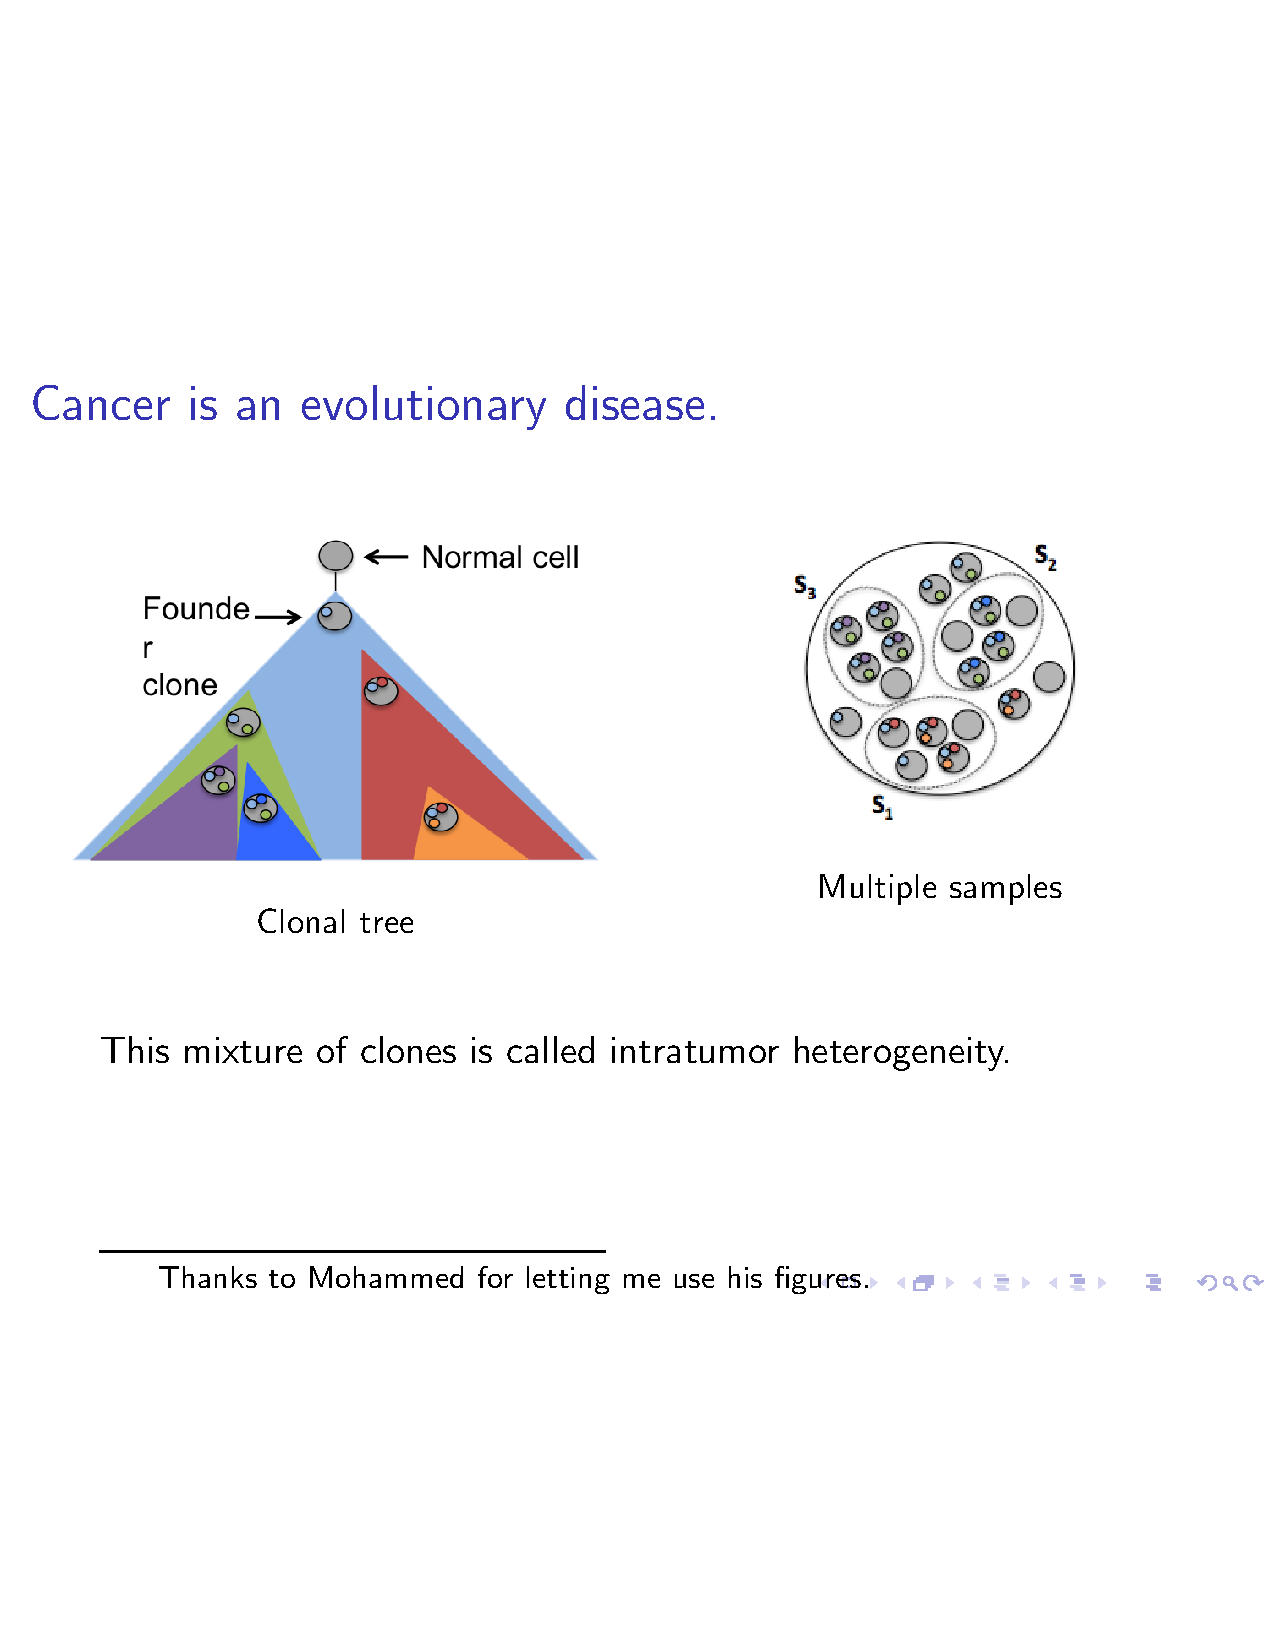
\includegraphics[page=1, width=\paperwidth]{DDL-UTRA-2016-intro.pdf}
\end{frame}

% Slide 3
\begin{frame}
\vspace*{-3.5cm}
\hspace*{-1.17cm}
\includegraphics[page=2, width=\paperwidth]{DDL-UTRA-2016-intro.pdf}
\end{frame}

% Slide 4
\begin{frame}
\vspace*{-3.5cm}
\hspace*{-1.17cm}
\includegraphics[page=3, width=\paperwidth]{DDL-UTRA-2016-intro.pdf}
\end{frame}

% Slide 5
\begin{frame}
\vspace*{-3.5cm}
\hspace*{-1.17cm}
\includegraphics[page=4, width=\paperwidth]{DDL-UTRA-2016-intro.pdf}
\end{frame}

% Slide 6
\begin{frame}
\vspace*{-3.5cm}
\hspace*{-1.17cm}
\includegraphics[page=5, width=\paperwidth]{DDL-UTRA-2016-intro.pdf}
\end{frame}

% Slide 7: Generative model, description
\begin{frame}{Model, Inference, Equations}
I will defer to the pdf here.
\end{frame}


%
%% Slide 7: Generative model, description
%\begin{frame}{Generative model for the data}
%
%\end{frame}
%
%% Slide 8: Generative model, graphical model
%\begin{frame}{Generative model for the data}
%
%\end{frame}
%
%% Slide 9: Generative model, equations
%\begin{frame}{Generative model for the data}
%
%\end{frame}
%
%% Slide 10: The goal of inference
%\begin{frame}{Goal of inference}
%
%\end{frame}
%
%% Slide 11: Variational inference, high level
%\begin{frame}{Variational inference}
%
%\end{frame}
%
%% Slide 11, Variational inference: KL Divergence, ELBO
%\begin{frame}{The ELBO}
%
%\end{frame}
%
%% Slide 11, Variational inference: Mean field parameterization of posterior
%\begin{frame}{Mean field parameterization}
%
%\end{frame}
%
%% Slide 12, Factorization
%\begin{frame}{Factorizing the posterior}
%So we want to minimize the ELBO.
%\end{frame}
%
%% Slide 13, Coordinate ascent
%\begin{frame}{Coordinate ascent}
%
%\end{frame}
%
%% Slide 14, Update equations for Multivariate binomial
%\begin{frame}{Update equations for the Multivariate binomial model}
%Exponential form makes this easy.
%\end{frame}
%
%% Slide 15, Update equations for Multivariate binomial
%\begin{frame}{Update equations for the Multivariate binomial model}
%Write them down. These are a pain to derive.
%\end{frame}
%
%% Slide 16, Update equations for Multivariate binomial
%\begin{frame}{Update equations for the Multivariate binomial model}
%Write them down.
%\end{frame}
%
%% Slide 17, Update equations for Multivariate binomial
%\begin{frame}{Update equations for the Multivariate binomial model}
%Write them down.
%\end{frame}
%
%% Slide 18, Implementation
%\begin{frame}{Implementation}
%In Python.
%\end{frame}

% Slide 19 to end, results
\begin{frame}
\vspace*{-3.5cm}
\hspace*{-1.17cm}
\includegraphics[page=6, width=\paperwidth]{DDL-UTRA-2016-intro.pdf}
\end{frame}

% Slide 20: Results
\begin{frame}
\vspace*{-3.5cm}
\hspace*{-1.17cm}
\includegraphics[page=7, width=\paperwidth]{DDL-UTRA-2016-intro.pdf}
\end{frame}

% Slide 21, plots
\begin{frame}{Plots}
\begin{itemize}
	\item Violin plots
	\item Posterior plots
\end{itemize}
\end{frame}

\end{document}